\section{System Architecture}

From the user point of view, our system is divided into two components: developers mode for training gestures and end-user mode for real-time prediction. In a high-level overview, developers using the developer mode supply the system with labeled data by wearing color gloves. Hence the developers hand the labeled image for the system to train. In the end-user mode, the users offer the raw image by showing up their hands, and the system will make predictions on every pixel using GPU and then pool every prediction to get an estimation of the gesture. Between the two modes, they share a component: feature extraction, which obtains the features for each pixel in the depth image. The implementation of feature extraction in the two modes are however different one is using CPU in an off-line fashion and the other is using GPU (end-user mode) in an on-demand fashion. 


%There are three main stages to our system. First is acquiring training samples using a colored glove. Second is training a classifier on the samples. Third is live prediction and pooling. 

%The approach is pixel-level classification, and future pooling. The motivation for pixel-level classification is the potential of parallelizing the task and using the GPU to achieve real-time prediction. 

\begin{figure}
\centering
	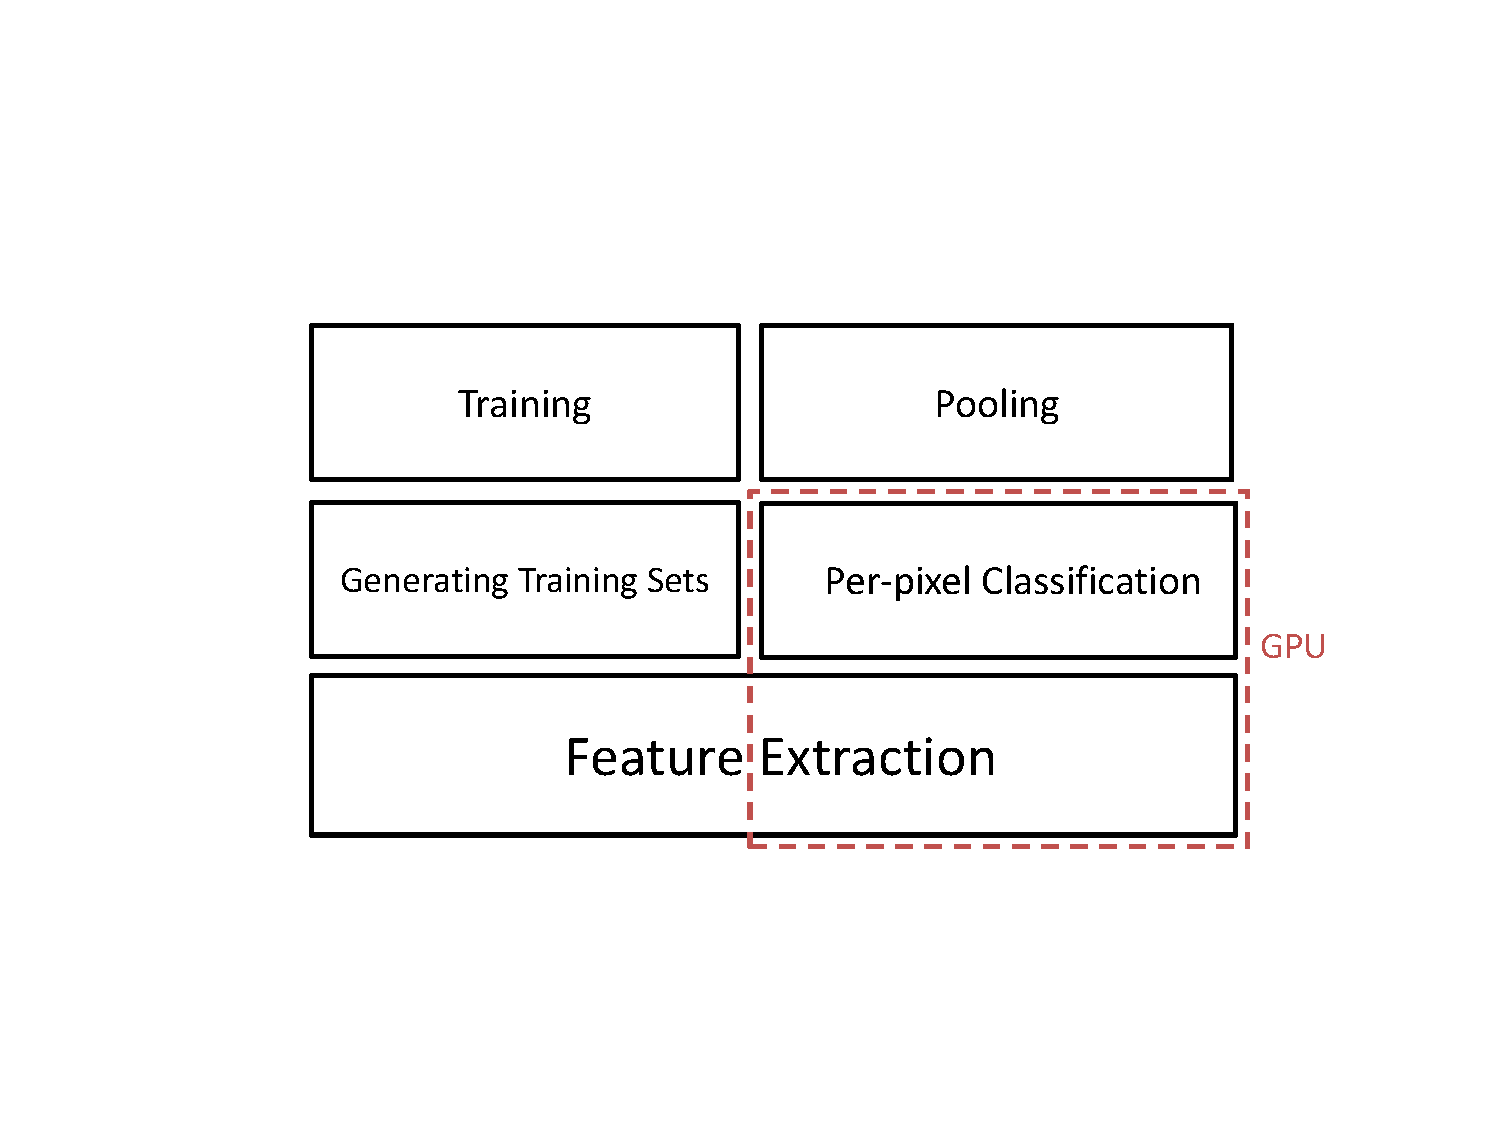
\includegraphics[width=0.5\textwidth]{fig/SystemArchitecture.pdf}
	\caption{An overview of the system architecture}
\label{fig: architecture}
\end{figure}

In the following, we go through feature extraction and per-pixel classification in Sec. X, generating training samples in Sec. Y, pooling in Sec. Z, and experiment in Sec. XX.